\chapter{Introdução}\label{intro}
\section{Justificativa}\label{sub:just}    

O ácido acetilsalicílico é, possivelmente, o medicamento mais conhecido e vendido no mundo atodo
Desse modo, a análise dos comprimidos comercializados é de interesse dos estudantes da Engenharia Química,
uma vez que proporciona aprendizado a cerca da indústria farmacêutica, padrões de qualidade, além de
práticas laboratoriais da teoria de química analítica e orgânica.

\section{Objetivos}\label{sub:Objetivos}
Determinar o teor de ácido acetilsalicílico contido nos comprimidos comercializados, analisando
medicamentos de referência (Aspirina$^{\tiny{\textregistered}}$), genéricos e similares.

\section{Referencial Teórico}\label{sub:reft}

\subsection{Histórico}\label{sub:Histórico}

O ácido acetilsalicílico (AAS) é um dos medicamentos mais populares no mundo, sendo conhecido por seu nome
comercial: Aspirina$^{\tiny{\textregistered}}$. Ele é um analgésico, anti-inflamatório e antipirético
produto de uma reação que tem como um dos reagentes o ácido salicílico, extraído do salgueiro (\textit{Salix
    alba}).  

O ácido acetilsalicílico pode ser identificado também pela sua fórmula química \ce{C9H8O4} e seu nome IUPAC
ácido 2-acetóxibenzóico. A respeito de propriedades físico-químicas, o AAS é um pó cristalino branco,
inodoro, solúvel em álcool e éter e pouco solúvel em água, possui ponto de fusão 135ºC e ponto de ebulição
a 140ºC. Ecologicamente, é facilmente biodegradado em estações de tratamento de água e não bioacumula.
\cite{teves}

A utilização do ácido salicílico, no alívio de dores já existe há séculos, isso porque essa ncia está
contida em diversas plantas consideradas medicinais. “Uma coleção de anotações datadas de cerca de 1500
a.C., conhecidas como papiros de Ebers, já recomendava o uso da infusão de folhas de murta para o alívio
de dores reumáticas” \cite{aspirinabayer}. Posteriormente, no século V a.C., Hipócrates, o pai da medicina
moderna, registrou que o pó da casca do salgueiro era capaz de amenizar dores e febre. Somente em 1860 a
ncia encontrada na casca do salgueiro foi isolada em laboratório e recebeu o nome de salicilato, que
designa um “grupo de fármacos que atuam devido ao seu conteúdo de ácido salicílico”. \cite{Goodman2005}

Já o descobrimento do ácido acetilsalicílico ocorreu mais tarde, “quando o químico alemão
Felix Hoffman pesquisava um medicamento para ser usado no tratamento da artrite, doença de seu pai. O
objetivo dele era encontrar uma droga para substituir o salicilato de sódio, medicamento usado naquela
época, mas que exigia grandes doses diárias e provocava irritação e fortes dores estomacais nos pacientes”
\cite{massabni2006}.

Em 1897, Hoffman, que trabalhava na companhia Bayer da Alemanha, preparou o ácido
acetilsalicílico combinando o ácido salicílico com acetato. A reação resultou numa ncia mais vantajosa do
que o salicilato de sódio, em questão de eficiência e efeitos colaterais. Tal droga recebeu,
posteriormente, o nome de Aspirina$^{\tiny{\textregistered}}$ e se tornou o primeiro fármaco sintetizado
em laboratório.  

A Aspirina$^{\tiny{\textregistered}}$ teve sua patente concedida em 1899 e começou a ser comercializada.
Ainda que inicialmente os superiores de Hoffman achassem que o medicamento fracassaria, o mesmo tornou-se
sucesso de vendas e inclusive destacou-se como medicamento mais utilizado no tratamento da artrite.
Inicialmente, a Aspirina$^{\tiny{\textregistered}}$
era vendida na forma de pó, entretanto, em 1900, ela tornou-se o primeiro medicamento no mundo a ser
vendido em doses padronizadas, que eram comprimidos com 500mg de ácido acetilsalicílico. “A formulação em
comprimidos tinha três vantagens principais: assegurar que cada comprimido tivesse uma dose exata do
ingrediente ativo, acabar com as falsificações dos produtos e reduzir os custos de
produção".\cite{aspirinabayer}

Décadas depois, John Vane, Professor de Farmacologia do London Royal College for Surgeons, “observou que
alguns tipos de ferimento eram acompanhados da liberação em nosso corpo de ncias chamadas de
prostaglandinas. Ele também percebeu que dois grupos delas provocavam febre e vermelhidão no local do
ferimento (sinais de inflamação). Vane e colaboradores descobriram que a
Aspirina$^{\tiny{\textregistered}}$ bloqueava a síntese de prostaglandinas, evitando a formação de
plaquetas, que depois se transformavam em coágulos de sangue no corpo humano. Esses coágulos eram
responsáveis pelo bloqueio do fluxo de sangue para o coração, resultando no ataque cardíaco. Assim, a
Aspirina$^{\tiny{\textregistered}}$ evita a formação de coágulos e, portanto, pode impedir o infarto do
miocárdio” \cite{massabni2006}. Em 1971, Vane publicou no jornal “Nature” seus estudos sobre o mecanismo de
ação do ácido acetilsalicílico, as descobertas feitas por ele lhe renderam o Prêmio Nobel de Medicina de
1982. 

Nos últimos 30 anos, pesquisa foram feitas com diferentes grupos de pessoas que apresentavam problemas
cardiovasculares, cerebrovasculares e também pessoas sadias. Os resultados mostraram que a
Aspirina$^{\tiny{\textregistered}}$ teve um grande impacto no tratamento e prevenção das doenças
cardiovasculares.  Além disso, pelo fato de ser anticoagulante, há trabalhos que mostram que a
Aspirina$^{\tiny{\textregistered}}$ reduz o risco de trombose e derrame cerebral. No entanto, algumas
pessoas podem apresentar efeitos colaterais como dores estomacais, diarréias, náuseas, sangramento e
hemorragia interna. Não é recomendado a sua utilização para quem possui problemas renais ou gástricos.

\subsection{Síntese de ácido acetilsalicílico}

A síntese da Aspirina$^{\tiny{\textregistered}}$ é dada através de uma reação de acetilação do ácido
salicílico, que é um composto aromático bifuncional, possuindo os grupos fenol e ácido carboxílico. A
acetilação ou etanoilação é o processo de introdução do grupo acetila (ou etanoila) em um composto
orgânico.

\begin{figure}[H]
\begin{center}
    
\includegraphics[width=.4\textwidth]{figuras/im1.png}
\end{center}
\caption{Grupo acetila ligado a uma cadeia carbônica.}\label{fig:im1}
\end{figure}

O radical acetila possui o grupo metila (\ce{CH3}-) conectado por uma ligação simples a um carbonila. O
carbono do grupo carbonila possui um único elétron livre, com o qual forma uma ligação com o radical R da
molécula.

A reação de acetilação do ácido salícilico é dada através do ataque nucleofilico do grupo -OH fenólico
sobre o carbono carbonílico do anidro acético, e, em seguida, da eliminação do ácido acético, que acaba
sendo um subproduto desta reação. “O oxigênio agora com três ligações desprotona reestabelecendo as duas
ligações e também reestabelecendo a acidez do meio, caracterizando um mecanismo de substituição
eletrofílica” \cite{lopes2011}. Do ponto de vista comercial, é proveitoso a utilização de um catalisador
como o ácido sulfúrico para a reação de esterificação. \cite{PERUCH2013}

\begin{figure}[H]
\begin{center}
    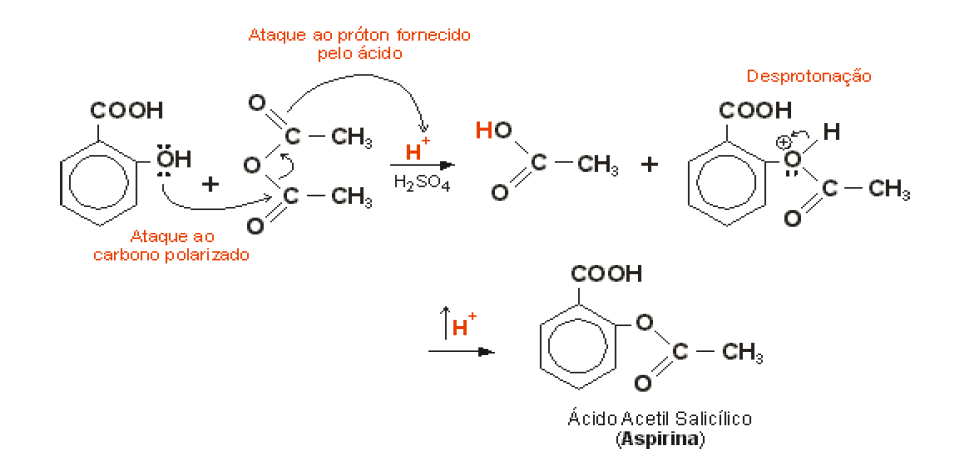
\includegraphics[width=1.2\textwidth]{figuras/im2.png}
\end{center}
\caption{Reação de síntese do ácido acetilsalicílico}\label{fig:im2}%
\end{figure}

\subsection{Mecanismo de ação da Aspirina}

 O ácido acetilsalicílico é um anti-inflamatório não esteroide (AINEs) ou não hormonal (AINHs), tendo como       propriedades analgésica, antipirética e anti-inflamatória. Além disso, possui um efeito inibitório sobre
as plaquetas no sangue e apresenta uma redução de 40\% no infarto do miocárdio fatal e não fatal (Palomo
et al., 2008).

É usado para o alívio da dor e de quadros febris, tais como resfriados e gripes, para controle da
temperatura e alívio das dores musculares e das articulações. Também é usado nos distúrbios inflamatórios
agudos e crônicos, tais como artrite reumatoide, osteoartrite e espondilite
anquilosante.\cite{bulaaspirina}

A atuação do ácido acetilsalicílico no organismo é de coibir a ação da ciclo-oxigenase. Essa ação utiliza
as enzimas COX-1 e COX-2, as quais transformam o ácido araquidônico em prostaglandinas, que são
responsáveis por induzir a dor e a febre. Esse ácido araquidônico é oriundo da ação enzimática da
Fosfolipase A2 sobre os fosfolipídios presentes nas membranas celulares. 

A plaqueta, importantíssima no processo de coagulação, é rica em COX-1 que, quando necessário, produz
prostaglandinas que são convertidas em Tramboxane A2 levando à formação de um coágulo. O processo de
coagulação se finda quando a Aspirina$^{\tiny{\textregistered}}$ age na inflamação. Com o cessar da ação
da Aspirina$^{\tiny{\textregistered}}$ no organismo, o processo de coagulação é retomado. Porém, uma vez
que as plaquetas não possuem núcleos elas não podem sintetizar uma nova COX para substituir a que foi
inativa pela Aspirina$^{\tiny{\textregistered}}$. Daí a ação anti-agregante plaquetária, que é um efeito
irreversível. Entretanto, essa ação irreversível não ocorre no endotélio vascular, pois este tem a
capacidade de sintetizar as novas moléculas. 

Devido a esse efeito inibitório da agregação plaquetária, o ácido acetilsalicílico pode aumentar a
tendência de sangramentos durante e após intervenções cirúrgicas (inclusive cirurgias de pequeno porte,
como por exemplo, extrações dentárias) \cite{bulaaspirina}.

Ademais, ao inibir a COX-2 ocorrerá o efeito anti-inflamatório, que diminuirá a inflamação vascular no
sítio da placa ateromatosa e esta, por sua vez, reduz a infiltração de células mononucleares na placa de
ateroma \cite{Grassi2012}.

Algumas das funções das prostaglandinas estão na produção do muco estomacal, na coagulação sanguínea e na
manutenção da taxa de filtração glomerular nos rins. Como o fármaco (ácido acetilsalicílico) inibe as
enzimas COXs não há a produção das prostaglandinas, tendo como consequências alguns efeitos no organismo.
Tais como, a úlcera péptica e uma posterior hemorragia digestiva, dependendo da gravidade do quadro; a
insuficiência renal aguda e problemas na coagulação. 

Após a medicação por via oral, o ácido acetilsalicílico é absorvido de forma rápida e completa no trato
gastrintestinal. Depois de absorvido e durante a sua absorção, o ácido acetilsalicílico é convertido em
ácido salicílico, que é o seu principal metabólito ativo. A quantidade máxima de fármaco na corrente
sanguínea do ácido acetilsalicílico é atingida após 10 a 20 minutos e a do ácido salicílico após 0,3 a 2
horas. 

O ácido acetilsalicílico e o ácido salicílico possuem uma grande afinidade com as proteínas plasmáticas,
logo eles ligam-se extensivamente com tais proteínas e são distribuídos por todo o organismo rapidamente.
O ácido salicílico passa para o leite materno e atravessa a placenta.

O ácido salicílico é eliminado principalmente por metabolismo hepático. Seus metabólitos incluem o ácido
salicilúrico, o glicuronídeo salicílico fenólico, o glicuronídeo salicilacílico, o ácido gentísico e o
ácido gentisúrico.

O metabolismo é restringido pela capacidade das enzimas hepáticas, sendo assim a cinética da eliminação
do ácido salicílico é dose-dependente. “A meia-vida de eliminação varia de 2 a 3 horas após doses baixas
até cerca de 15 horas com doses altas” \cite{bulaaspirina}. O ácido salicílico e seus metabólicos são
excretados predominantemente por via renal. 

É importante frisar que esses anti-inflamatórios não esteroides (AINEs), do qual o ácido acetilsalicílico
faz parte, apenas inibem a produção de prostaglandinas na inflamação, mas eles não cessam a mesma.

\subsection{Medicamentos de referência, genéricos e similares}\label{refgensim}

No mercado farmacêutico, medicamentos com o mesmo princípio ativo podem surgir com diferentes marcas ou
classificações. No caso do ácido acetilsalicílico, algumas são associadas a outras ncias como cafeína ou
vitamina C.Outras possuem revestimentos de cápsula que buscam diminuir a agressão ao sistema digestivo.
\cite{prade2006}

Com essas diferenças, os remédios são classificados como referência, genérico e similar. Os medicamentos
de referência, que também são conhecidos como “de marca”, são remédios que possuem eficiência
terapêutica, com qualidade e seguranças comprovadas cientificamente. São registrados juntamente à Agência
Nacional de ncia Sanitária. Geralmente são medicamentos com novos princípios ativos o que trazem
novidades para o tratamento da doença

Com essas diferenças, os remédios são classificados como referência, genérico e similar. Os medicamentos
de referência, que também são conhecidos como “de marca”, são remédios que possuem eficiência
terapêutica, com qualidade e seguranças comprovadas cientificamente. São registrados juntamente à Agência
Nacional de ncia Sanitária. Geralmente são medicamentos com novos princípios ativos o que trazem
novidades para o tratamento da doença.

Já os similares, além de possuir o mesmo princípio ativo do medicamento de referência, possui uma
identificação de nome comercial ou marca. A diferença é apresentada em alguns aspectos como embalagem,
rótulo, tamanho, validade e forma do produto. De acordo com a regulamentação da ANVISA, dado uma
prescrição médica os medicamentos de referência não podem ser substituídos por similares.

Para a possibilidade de troca desses medicamentos, ou seja, serem intercambiáveis, eles devem apresentar
um dos três testes: bioequivalência, biodisponibilidade e bioisenção. O estudo de bioequivalência é
sempre realizado entre o medicamento de referência e o estudado. Estas análises tem o intuito de
reafirmar a igualdade entre os produtos, proporcionando segurança e eficiência. \cite{ache2015}

\subsection{Titulação}\label{titulacao}

``Titulação é um procedimento no qual a quantidade de analito de uma amostra é determinada
adicionando-se uma quantidade conhecida de um reagente que reage completamente com o analito de
uma forma bem definida'' (HAGE, CARR. 2012) \cite{Hage2012}.

Titulações volumétricas compreendem a medida de volume de uma solução padrão (de concentração
conhecida) necessária para reagir completamente com o analito. \cite{Skoog2014}

Em uma titulação ácido-base, o titulado (analito) é um ácido e o titulante (solução ou composto com
os metros conhecidos) é uma base, ou vice-versa.

Para saber quando e quanto de todo o analito reagiu, é necessário adicionar um indicador ácido-base,
uma ncia química que muda de cor em uma faixa conhecida de pH, ajudando a detectar o ponto
estequiométrico ou ponto de equivalência.

``O ponto de equivalência é o ponto teórico alcançado quando a quantidade adicionada do titulante é
quimicamente equivalente à quantidade de analito na amostra'' \cite{Skoog2014}. O ponto final é o
ponto onde ocorre visualmente a percepção de alterações físicas (cor ou turbidez) pelo observador.

“Entre o ponto final da titulação e o ponto estequiométrico (teórico) sempre existirá uma pequena
diferença de volume do titulante chamada de Erro de Titulação”. \cite{Ruy1999}

A reação de neutralização do AAS é dada abaixo:

\begin{center}
    \ce{C8O2H7COOH + NaOH -> C8O2H7COONa + H2O}
\end{center} 

\subsubsection{Titulação de ácido fraco com base forte}

Segundo Skoog et al. (2014), na titulação de um ácido fraco (HA) com uma base forte (\ce{NaOh} ou
\ce{KOH}) ocorrem as seguintes etapas:

\begin{enumerate}
    \item No início, a solução contém somente o analito, ácido fraco.
    \item Com a adição do titulante (até antes do ponto de equivalência), a solução contém uma série
        de tampões, entre a base conjugada formada da reação e o ácido fraco residual que permanece.
    \item No ponto de equivalência, a solução contém apenas o conjugado do ácido (um sal).
    \item Após o ponto de equivalência, o excesso de titulante básico reprime o caráter ácido ou
        alcalino do sal formado, produto da reação, sendo o pH resultante da concentração do excesso
        de titulante.
\end{enumerate}

\begin{figure}[H]
\begin{center}
    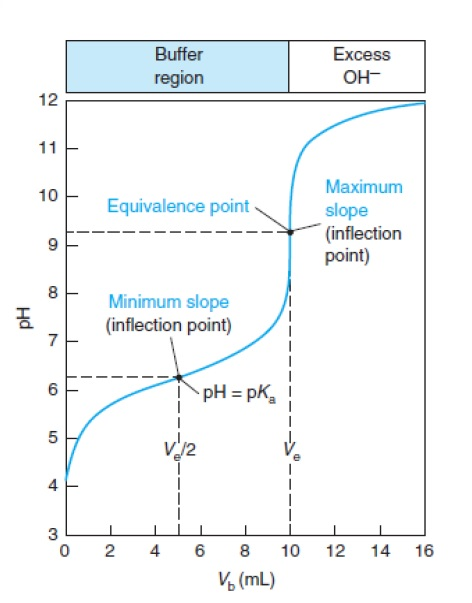
\includegraphics[scale=.9]{figuras/titulacao.jpg}
\end{center}
\caption{Curva de titulação Ácido fraco $\times$ Base forte}
\label{fig:curva_titulacao}
\end{figure}

